\documentclass[12pt,a4paper]{article}
\usepackage[utf8]{vietnam}
\usepackage{amsmath,amssymb}
\usepackage[a4paper,left=2cm,right=1.8cm,top=1.8cm,bottom=1.8cm]{geometry}
\usepackage{tikz}
\usepackage{array,tabularx,longtable}
\usepackage{enumitem}
\setlength{\parindent}{0pt}
\setlength{\parskip}{3pt}
\linespread{1.15}
\pagestyle{plain}

% Phương án trắc nghiệm: 4 phương án trên 1 dòng / 2 dòng / mỗi phương án 1 dòng
\newcommand{\bonpa}[4]{\par\noindent\begin{tabularx}{\linewidth}{@{\hspace{0.6cm}}XXXX@{}}
\textbf{A.} #1 & \textbf{B.} #2 & \textbf{C.} #3 & \textbf{D.} #4\end{tabularx}\par}
\newcommand{\haipa}[4]{\par\noindent\begin{tabularx}{\linewidth}{@{\hspace{0.6cm}}XX@{}}
\textbf{A.} #1 & \textbf{B.} #2\\ \textbf{C.} #3 & \textbf{D.} #4\end{tabularx}\par}
\newcommand{\motpa}[4]{\par\hspace*{0.6cm}\textbf{A.} #1\par\hspace*{0.6cm}\textbf{B.} #2\par
\hspace*{0.6cm}\textbf{C.} #3\par\hspace*{0.6cm}\textbf{D.} #4\par}
\newcommand{\cau}[1]{\par\medskip\textbf{Câu #1.}~}
\newcommand{\bai}[2]{\par\medskip\textbf{Bài #1} \textit{(#2)}.~}
\newcommand{\y}[1]{\par\hspace*{0.6cm}#1}
\newcommand{\phan}[1]{\par\bigskip{\large\textbf{#1}}\par\smallskip}
\setlength{\extrarowheight}{2pt}

\begin{document}
% ===================== ĐỀ SỐ 1 =====================
\noindent
\begin{minipage}[t]{0.38\linewidth}\centering
TRƯỜNG THCS \dotfill\\[2pt]
\textbf{ĐỀ SỐ 1}
\end{minipage}\hfill
\begin{minipage}[t]{0.6\linewidth}\centering
\textbf{ĐỀ KIỂM TRA GIỮA HỌC KÌ I}\\
\textbf{NĂM HỌC 2026 -- 2027}\\
\textbf{MÔN: TOÁN 7} -- Sách \textit{Kết nối tri thức với cuộc sống}\\
\textit{Thời gian làm bài: 90 phút (không kể thời gian giao đề)}
\end{minipage}

\medskip
Họ và tên: \dotfill\ Lớp: \makebox[2cm]{\dotfill}\ Số báo danh: \makebox[2.5cm]{\dotfill}
\phan{A. TRẮC NGHIỆM (3,0 điểm)}
\textbf{Phần I. Câu trắc nghiệm nhiều phương án lựa chọn} \textit{(1,0 điểm)}. Thí sinh trả lời từ câu 1 đến câu 4. Mỗi câu hỏi thí sinh chỉ chọn một phương án.
\cau{1} Số nào sau đây là số hữu tỉ âm?
\bonpa{$\dfrac{-3}{-5}$}{$0$}{$\dfrac{2}{-7}$}{$\dfrac{-4}{-9}$}
\cau{2} Kết quả của phép tính $\left(-\dfrac{2}{3}\right)^{3}$ là
\bonpa{$-\dfrac{8}{27}$}{$\dfrac{8}{27}$}{$-\dfrac{6}{9}$}{$-\dfrac{8}{9}$}
\cau{3} Phân số nào sau đây viết được dưới dạng số thập phân vô hạn tuần hoàn?
\bonpa{$\dfrac{3}{8}$}{$\dfrac{7}{20}$}{$\dfrac{5}{12}$}{$\dfrac{9}{25}$}
\cau{4} Cho hai đường thẳng $xx'$ và $yy'$ cắt nhau tại $O$. Biết $\widehat{xOy}=50^\circ$. Số đo của $\widehat{x'Oy'}$ là
\bonpa{$50^\circ$}{$130^\circ$}{$40^\circ$}{$180^\circ$}

\medskip\textbf{Phần II. Câu trắc nghiệm đúng sai} \textit{(1,0 điểm)}. Trong mỗi ý a), b), c), d) ở câu 5, thí sinh chọn đúng hoặc sai.
\cau{5} Cho hai số hữu tỉ $x=-\dfrac{3}{4}$ và $y=\dfrac{1}{2}$.
\y{a) $x\cdot y=\dfrac{3}{8}$.}
\y{b) $x<y$.}
\y{c) Số đối của $x$ là $\dfrac{4}{3}$.}
\y{d) $x+y=-\dfrac{1}{4}$.}

\medskip\textbf{Phần III. Câu trắc nghiệm trả lời ngắn} \textit{(1,0 điểm)}. Thí sinh trả lời từ câu 6 đến câu 9.
\cau{6} Tính giá trị của biểu thức $\dfrac{3^{5}}{3^{3}}-\left(\dfrac{1}{2}\right)^{0}$.
\cau{7} Tìm $x$, biết $x-\dfrac{1}{3}=\dfrac{2}{3}$.
\cau{8} Cho tam giác $ABC$ có $\widehat{A}=80^\circ$, $\widehat{B}=45^\circ$. Tính số đo $\widehat{C}$ (đơn vị: độ).
\cau{9} Cho tia $Oz$ là tia phân giác của $\widehat{xOy}$, biết $\widehat{xOy}=120^\circ$. Tính số đo $\widehat{xOz}$ (đơn vị: độ).
\phan{B. TỰ LUẬN (7,0 điểm)}
\bai{1}{1,0 điểm} Tính (hợp lí nếu có thể):
\par\noindent\begin{tabularx}{\linewidth}{@{\hspace{0.6cm}}XX@{}}a) $\dfrac{5}{9}\cdot\dfrac{-3}{7}+\dfrac{5}{9}\cdot\dfrac{-4}{7}$; & b) $\left(-\dfrac{1}{2}\right)^{2}+\dfrac{3}{4}:\dfrac{3}{2}-1{,}5$.\end{tabularx}
\bai{2}{1,5 điểm} Tìm $x$, biết:
\y{a) $x+\dfrac{2}{3}=-\dfrac{1}{6}$;}
\y{b) $\dfrac{3}{4}-2x=\dfrac{1}{4}$;}
\y{c) $\left(x-\dfrac{1}{2}\right)^{2}=\dfrac{9}{16}$.}
\bai{3}{1,0 điểm} Một cửa hàng có $150$ kg gạo. Ngày thứ nhất cửa hàng bán được $\dfrac{2}{5}$ số gạo. Ngày thứ hai cửa hàng bán được $\dfrac{3}{4}$ số gạo còn lại. Hỏi sau hai ngày, cửa hàng còn lại bao nhiêu ki-lô-gam gạo?
\bai{4}{1,5 điểm} Cho hình vẽ bên, đường thẳng $c$ cắt hai đường thẳng $a$ và $b$ lần lượt tại $A$ và $B$. Biết $\widehat{A_1}=115^\circ$, $\widehat{B_1}=65^\circ$.
\begin{center}
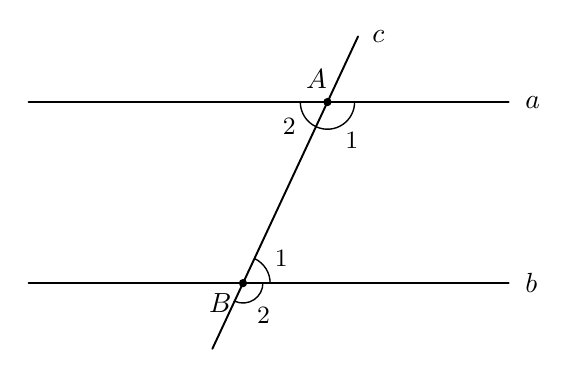
\begin{tikzpicture}[scale=1.15,line cap=round,line join=round]
  \draw[line width=0.7pt] (-0.300,2.000) -- (5.000,2.000);
  \draw[line width=0.7pt] (-0.300,0.000) -- (5.000,0.000);
  \draw[line width=0.7pt] (3.338,2.725) -- (1.729,-0.725);
  \node[anchor=west,inner sep=1pt] at (5.150,2.000) {$a$};
  \node[anchor=west,inner sep=1pt] at (5.150,0.000) {$b$};
  \node[anchor=west,inner sep=1pt] at (3.458,2.725) {$c$};
  \fill (3.000,2.000) circle (1.3pt);
  \node[anchor=center,inner sep=1pt] at (2.880,2.250) {$A$};
  \fill (2.067,0.000) circle (1.3pt);
  \node[anchor=center,inner sep=1pt] at (1.817,-0.220) {$B$};
  \draw[line width=0.5pt] (2.873,1.728) arc[start angle=-115,end angle=0,radius=0.300];
  \node[anchor=center,inner sep=1pt] at (3.269,1.578) {{\small 1}};
  \draw[line width=0.5pt] (2.700,2.000) arc[start angle=-180,end angle=-115,radius=0.300];
  \node[anchor=center,inner sep=1pt] at (2.578,1.731) {{\small 2}};
  \draw[line width=0.5pt] (2.367,0.000) arc[start angle=0,end angle=65,radius=0.300];
  \node[anchor=center,inner sep=1pt] at (2.489,0.269) {{\small 1}};
  \draw[line width=0.5pt] (1.974,-0.199) arc[start angle=-115,end angle=0,radius=0.220];
  \node[anchor=center,inner sep=1pt] at (2.293,-0.354) {{\small 2}};
\end{tikzpicture}
\end{center}
\y{a) Chứng minh $a\parallel b$.}
\y{b) Tính số đo $\widehat{B_2}$.}
\y{c) Đường thẳng $d$ vuông góc với đường thẳng $a$. Chứng minh $d\perp b$.}
\bai{5}{1,5 điểm} Cho tam giác $ABC$ có $AB=AC$. Gọi $M$ là trung điểm của đoạn thẳng $BC$.
\y{a) Chứng minh $\triangle ABM=\triangle ACM$.}
\y{b) Chứng minh $AM$ là tia phân giác của $\widehat{BAC}$.}
\y{c) Chứng minh $AM\perp BC$.}
\bai{6}{0,5 điểm} Tính tổng $A=\dfrac{1}{1\cdot 2}+\dfrac{1}{2\cdot 3}+\dfrac{1}{3\cdot 4}+\ldots+\dfrac{1}{99\cdot 100}$.

\bigskip\begin{center}\textbf{--------- HẾT ---------}\\
\textit{Giáo viên coi kiểm tra không giải thích gì thêm.}\end{center}

\newpage
\begin{center}{\large\textbf{HƯỚNG DẪN CHẤM -- ĐỀ SỐ 1}}\end{center}
\phan{A. TRẮC NGHIỆM (3,0 điểm)}
\textbf{Phần I.} Mỗi câu trả lời đúng được 0,25 điểm.

\begin{tabular}{|l|*{4}{>{\centering\arraybackslash}p{2cm}|}}\hline
Câu & 1 & 2 & 3 & 4 \\ \hline
Đáp án & \textbf{C} & \textbf{A} & \textbf{C} & \textbf{A} \\ \hline
\end{tabular}

\textbf{Phần II.} Mỗi ý trả lời đúng được 0,25 điểm.

\begin{tabular}{|l|*{4}{>{\centering\arraybackslash}p{2cm}|}}\hline
Câu 5 & a) & b) & c) & d) \\ \hline
Đáp án & \textbf{Sai} & \textbf{Đúng} & \textbf{Sai} & \textbf{Đúng} \\ \hline
\end{tabular}

\textbf{Phần III.} Mỗi câu trả lời đúng được 0,25 điểm.

\begin{tabular}{|l|*{4}{>{\centering\arraybackslash}p{2cm}|}}\hline
Câu & 6 & 7 & 8 & 9 \\ \hline
Đáp án & \textbf{8} & \textbf{1} & \textbf{55} & \textbf{60} \\ \hline
\end{tabular}

\phan{B. TỰ LUẬN (7,0 điểm)}
\begin{longtable}{|>{\bfseries}c|p{0.76\linewidth}|>{\centering\arraybackslash}p{1.3cm}|}\hline
Bài & \multicolumn{1}{c|}{\textbf{Nội dung}} & \textbf{Điểm} \\ \hline\endhead
1a & \rule{0pt}{4ex}$\dfrac{5}{9}\cdot\dfrac{-3}{7}+\dfrac{5}{9}\cdot\dfrac{-4}{7}=\dfrac{5}{9}\cdot\left(\dfrac{-3}{7}+\dfrac{-4}{7}\right)$\rule[-2.4ex]{0pt}{0pt} & 0,25 \\ \hline
 & \rule{0pt}{4ex}$=\dfrac{5}{9}\cdot(-1)=-\dfrac{5}{9}$\rule[-2.4ex]{0pt}{0pt} & 0,25 \\ \hline
1b & \rule{0pt}{4ex}$\left(-\dfrac{1}{2}\right)^{2}+\dfrac{3}{4}:\dfrac{3}{2}-1{,}5=\dfrac{1}{4}+\dfrac{3}{4}\cdot\dfrac{2}{3}-\dfrac{3}{2}=\dfrac{1}{4}+\dfrac{1}{2}-\dfrac{3}{2}$\rule[-2.4ex]{0pt}{0pt} & 0,25 \\ \hline
 & \rule{0pt}{4ex}$=\dfrac{1}{4}-1=-\dfrac{3}{4}$\rule[-2.4ex]{0pt}{0pt} & 0,25 \\ \hline
2a & \rule{0pt}{4ex}$x=-\dfrac{1}{6}-\dfrac{2}{3}=-\dfrac{1}{6}-\dfrac{4}{6}$\rule[-2.4ex]{0pt}{0pt} & 0,25 \\ \hline
 & \rule{0pt}{4ex}$x=-\dfrac{5}{6}$. Vậy $x=-\dfrac{5}{6}$.\rule[-2.4ex]{0pt}{0pt} & 0,25 \\ \hline
2b & \rule{0pt}{4ex}$2x=\dfrac{3}{4}-\dfrac{1}{4}=\dfrac{1}{2}$\rule[-2.4ex]{0pt}{0pt} & 0,25 \\ \hline
 & \rule{0pt}{4ex}$x=\dfrac{1}{2}:2=\dfrac{1}{4}$. Vậy $x=\dfrac{1}{4}$.\rule[-2.4ex]{0pt}{0pt} & 0,25 \\ \hline
2c & \rule{0pt}{4ex}$\left(x-\dfrac{1}{2}\right)^{2}=\left(\dfrac{3}{4}\right)^{2}=\left(-\dfrac{3}{4}\right)^{2}$ nên $x-\dfrac{1}{2}=\dfrac{3}{4}$ hoặc $x-\dfrac{1}{2}=-\dfrac{3}{4}$\rule[-2.4ex]{0pt}{0pt} & 0,25 \\ \hline
 & \rule{0pt}{4ex}$x=\dfrac{5}{4}$ hoặc $x=-\dfrac{1}{4}$. Vậy $x\in\left\{\dfrac{5}{4};-\dfrac{1}{4}\right\}$.\rule[-2.4ex]{0pt}{0pt} & 0,25 \\ \hline
3 & \rule{0pt}{4ex}Số gạo bán ngày thứ nhất: $150\cdot\dfrac{2}{5}=60$ (kg).\rule[-2.4ex]{0pt}{0pt} & 0,25 \\ \hline
 & Số gạo còn lại sau ngày thứ nhất: $150-60=90$ (kg). & 0,25 \\ \hline
 & \rule{0pt}{4ex}Số gạo bán ngày thứ hai: $90\cdot\dfrac{3}{4}=67{,}5$ (kg).\rule[-2.4ex]{0pt}{0pt} & 0,25 \\ \hline
 & Số gạo còn lại sau hai ngày: $90-67{,}5=22{,}5$ (kg). & 0,25 \\ \hline
4a & Ta có $\widehat{A_1}+\widehat{A_2}=180^\circ$ (hai góc kề bù) nên $\widehat{A_2}=180^\circ-115^\circ=65^\circ$. & 0,25 \\ \hline
 & Do đó $\widehat{A_2}=\widehat{B_1}=65^\circ$, mà $\widehat{A_2}$ và $\widehat{B_1}$ ở vị trí so le trong nên $a\parallel b$. & 0,25 \\ \hline
4b & $\widehat{B_1}$ và $\widehat{B_2}$ là hai góc kề bù nên $\widehat{B_1}+\widehat{B_2}=180^\circ$ & 0,25 \\ \hline
 & $\widehat{B_2}=180^\circ-65^\circ=115^\circ$. & 0,25 \\ \hline
4c & Ta có $d\perp a$ và $a\parallel b$ & 0,25 \\ \hline
 & nên $d\perp b$ (một đường thẳng vuông góc với một trong hai đường thẳng song song thì vuông góc với đường thẳng kia). & 0,25 \\ \hline
5 & Vẽ hình, ghi GT – KL đúng. \newline \textit{(Hình vẽ ở cuối hướng dẫn chấm)} & 0,25 \\ \hline
5a & Xét $\triangle ABM$ và $\triangle ACM$ có: $AB=AC$ (gt); $BM=CM$ ($M$ là trung điểm $BC$); $AM$ là cạnh chung. & 0,25 \\ \hline
 & Do đó $\triangle ABM=\triangle ACM$ (c.c.c). & 0,25 \\ \hline
5b & Vì $\triangle ABM=\triangle ACM$ nên $\widehat{BAM}=\widehat{CAM}$ (hai góc tương ứng). Mà tia $AM$ nằm giữa hai tia $AB$, $AC$ nên $AM$ là tia phân giác của $\widehat{BAC}$. & 0,25 \\ \hline
5c & Vì $\triangle ABM=\triangle ACM$ nên $\widehat{AMB}=\widehat{AMC}$ (hai góc tương ứng). Mà $\widehat{AMB}+\widehat{AMC}=180^\circ$ (hai góc kề bù) & 0,25 \\ \hline
 & nên $\widehat{AMB}=\widehat{AMC}=90^\circ$. Vậy $AM\perp BC$. & 0,25 \\ \hline
6 & \rule{0pt}{4ex}$A=\left(1-\dfrac{1}{2}\right)+\left(\dfrac{1}{2}-\dfrac{1}{3}\right)+\ldots+\left(\dfrac{1}{99}-\dfrac{1}{100}\right)$ (vì $\dfrac{1}{n(n+1)}=\dfrac{1}{n}-\dfrac{1}{n+1}$)\rule[-2.4ex]{0pt}{0pt} & 0,25 \\ \hline
 & \rule{0pt}{4ex}$A=1-\dfrac{1}{100}=\dfrac{99}{100}$.\rule[-2.4ex]{0pt}{0pt} & 0,25 \\ \hline
\end{longtable}
\textit{Lưu ý: Học sinh làm cách khác đúng vẫn cho điểm tối đa theo thang điểm tương ứng. Bài hình không vẽ hình hoặc vẽ hình sai không chấm phần tương ứng.}

\textbf{Hình vẽ bài 5:}
\begin{center}
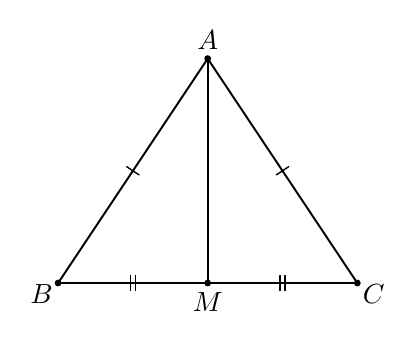
\begin{tikzpicture}[scale=0.95,line cap=round,line join=round]
  \draw[line width=0.7pt] (2.000,3.000) -- (0.000,0.000);
  \draw[line width=0.7pt] (2.000,3.000) -- (4.000,0.000);
  \draw[line width=0.7pt] (0.000,0.000) -- (4.000,0.000);
  \draw[line width=0.7pt] (2.000,3.000) -- (2.000,0.000);
  \draw[line width=0.5pt] (0.917,1.555) -- (1.083,1.445);
  \draw[line width=0.5pt] (2.917,1.445) -- (3.083,1.555);
  \draw[line width=0.5pt] (0.965,-0.100) -- (0.965,0.100);
  \draw[line width=0.5pt] (1.035,-0.100) -- (1.035,0.100);
  \draw[line width=0.5pt] (2.965,-0.100) -- (2.965,0.100);
  \draw[line width=0.5pt] (3.035,-0.100) -- (3.035,0.100);
  \fill (2.000,3.000) circle (1.3pt);
  \node[anchor=center,inner sep=1pt] at (2.000,3.250) {$A$};
  \fill (0.000,0.000) circle (1.3pt);
  \node[anchor=center,inner sep=1pt] at (-0.220,-0.150) {$B$};
  \fill (4.000,0.000) circle (1.3pt);
  \node[anchor=center,inner sep=1pt] at (4.220,-0.150) {$C$};
  \fill (2.000,0.000) circle (1.3pt);
  \node[anchor=center,inner sep=1pt] at (2.000,-0.250) {$M$};
\end{tikzpicture}
\end{center}

\end{document}
